\subsubsection{概要}
Docker\cite{docker}は,アプリケーションの開発,導入,実行するためのオープンなプラットフォームである.
Dockerを利用すれば,アプリケーションをインフラストラクチャーから分離できるため,ソフトウェアを素早く提供できる.
また,Dockerはアプリケーションをパッケージ化して実行するために,ほぼ分離された環境となるコンテナを提供している.

\subsubsection{コンテナ}\label{sec:container}
コンテナはDockerがアプリケーションを実行するための,ほぼ分離された環境を提供する.
ほぼ分離された環境というものはnamespace\cite{namespace}で実現されている.

コンテナはnamespaceを用いることによって図\ref{namespace}のように作成されている.

\begin{figure}[htbp]
    \begin{center}
        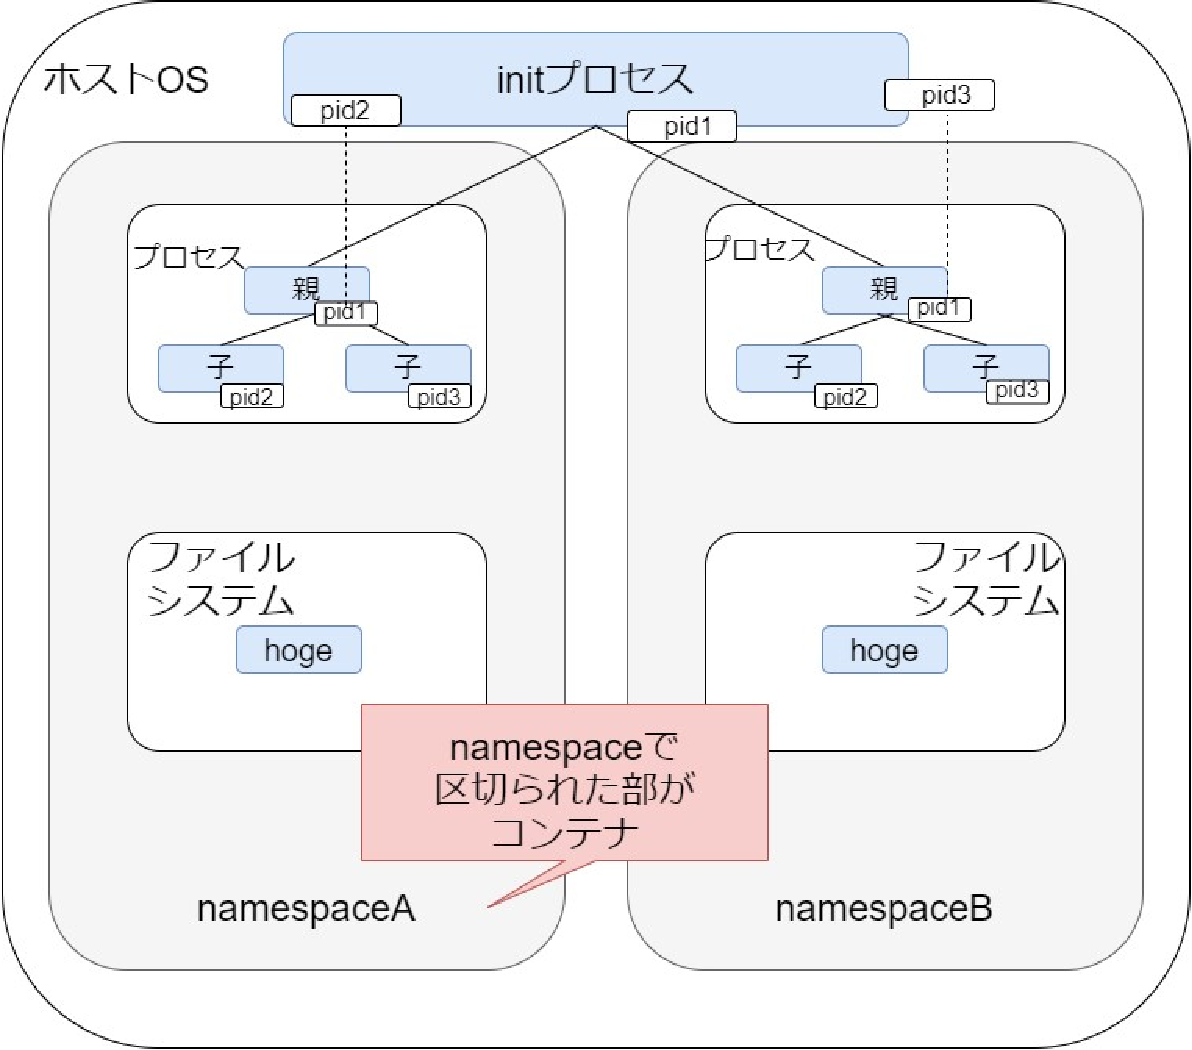
\includegraphics[width=13cm,height=12cm,keepaspectratio]{namespace-crop.pdf}\\
        %includegraphicsの詳しい使い方ははLaTeXの参考書を参照.
    \end{center}
    \caption{コンテナの構成図}
    \label{namespace}
\end{figure}

ホストOS上にnamespaceAとnamespaceBを作成し,それぞれのnamespaceの空間で全く独立したファイル構造やプロセス空間を持つことができる.
このように分離された環境をコンテナという.
コンテナのプロセス空間に関しては,実際にはホストOS上で動作しているプロセスIDとコンテナ上で動作しているプロセスIDをマッピングしているテーブルが存在する.
これを用いてホストOS上ではpid2として認識されているが,コンテナ上ではpid1として認識されていることになる.

このことによりnamespaceを利用すると,プロセス空間やファイルシステムを一つのOSの中で分離できるので,namespaceで区切られた部分であるコンテナは全く異なるOSのようにふるまうことが可能となる.

\subsubsection{Docker Engine}
\ref{sec:container}節で述べたようにDockerはコンテナを用いて動作している.
しかし,プロセスをコンテナ上で稼働させるためには,OSの動作に必要なコマンドやライブラリが必要になる.
これを実現するためには相当量のコマンドを発行しなければならない.
そこでDockerは,Docker Engineを作成した.
Docker Engineは主に以下のコンポーネントからなるクライアントサーバ型アプリケーションである.

\begin{description}
    \item[・サーバ]\mbox{}\\
        長時間稼働する種類のプログラムでありデーモン・プロセスと呼ばれる.
    \item[・REST API]\mbox{}\\
        プログラムとデーモンとの間での通信方法を定義し,何をなすべきかを指示する.
    \item[・コマンドライン・インターフェイス(CLI)]\mbox{}\\
        クライアント.dockerコマンドなど.
\end{description}

デーモンは,Dockerオブジェクトを作成,管理する.
Dockerオブジェクトとは,イメージ,コンテナ,ネットワーク,データ,ボリュームなどを表す.

CLIはDocker REST APIを通じて,スクリプトのコマンド実行により,Dockerデーモンを制御,入出力を実行する.
Dockerアプリケーションの多くが,基本的なところでこのAPIやCLIを利用している.

また,Dockerの内部には以下の3つのコンポーネントが存在する.

\begin{itemize}
    \item Dockerイメージ
    \item Dockerレジストリ
    \item Dockerコンテナ
\end{itemize}

Dockerイメージとは,読み込み専用なテンプレートである.
DockerイメージはDockerコンテナ作成時に使用される.
各イメージはレイヤの積み重ねで構成される.
また,新しいイメージの構築や既存のイメージの更新だけでなく,他人が作成したDockerイメージをダウンロードして使用することも可能である.
DockerはUnionFS\cite{Unionfs}を用いて各イメージのレイヤを単一のイメージに連結する.
これにより,Dockerイメージに変更を加えた場合,変更したい部分のレイヤを追加もしくは更新するだけでよいため,構築に時間がかからず早く簡単にイメージを提供できる.

Dockerレジストリとは,イメージを保持するものである.
パブリックもしくはプライベートに保管されているイメージのアップデートやダウンロードを実行することができる.
パブリックなDockerレジストリとしてDocker Hub\cite{dockerhub}が提供されている.

Dockerコンテナとは,ディレクトリと似たようなもので,アプリケーションの実行に必要なすべてが含まれている.
各コンテナはDockerイメージによって作成される.
Dockerコンテナは実行・開始・停止・移動・削除できる.
各コンテナは隔離されているため,安全なアプリケーションのプラットフォームとして動作する.


\subsubsection{Docker Compose}
Composeとは,複数のコンテナを定義し実行するDockerアプリケーションの為のツールである.
ComposeにおいてはYAML\cite{YAML}ファイルを使ってアプリケーションサービスの設定する.
コマンド一つ実行するだけで,設定内容に基づいたアプリケーションを生成,起動する.

Composeを使うには基本的に3つのステップを踏む.

\begin{enumerate}
    \item アプリケーション環境をDockerfileに定義する.
    \item アプリケーションを構成するサービスをdocker-compose.ymlファイル内に定義する.
    \item docker-compose upを実行したら,Composeはアプリケーション全体を起動・実行する.
\end{enumerate}

\newpage
\subsubsection{コマンド一覧}
DockerとDocker Composeで使用する代表的なコマンド一覧とコマンドの説明を表\ref{docker_command}に示す.


\begin{table}[htb]
    \begin{center}
        \caption{Dockerコマンド一覧}
        \begin{tabularx}{\textwidth}{|l|X|}\hline
            docker run -it [イメージ名] /bin/bash & dockerコンテナを起動し,ログイン \\ \hline
            docker run -p [外部ポート]:[コンテナポート] & コンテナに外部からアクセスする \\ \hline
            docker run -v [ホストボリュームパス]:[コンテナ内パス] [コンテナイメージ名] & コンテナのボリュームをホストにマウントする \\ \hline
            docker save [イメージ名] \textgreater [ファイル名].tar.gz & dockerイメージをtar.gz形式で保存する\\ \hline
            docker load \textless [ファイル名].tar.gz & tar.gz形式のdockerイメージを取り込む \\ \hline
            docker exec -it [コンテナID/コンテナ名] /bin/bash & 起動中のコンテナにログイン \\ \hline
            docker cp [ホストファイルパス] [コンテナID]:[コンテナコピー先パス] & 起動中コンテナにホストからファイルをコピー \\ \hline
            docker commit [起動中のコンテナID] [イメージ名] & 起動中のコンテナをイメージとして保存 \\ \hline
            docker start [コンテナ名] & コンテナの開始 \\ \hline
            docker stop [コンテナ名] & コンテナの停止 \\ \hline
            docker restart [コンテナ名] & コンテナの再起動 \\ \hline
        \end{tabularx}
        \label{docker_command}
    \end{center}
\end{table}


\begin{table}[htb]
    \begin{center}
        \caption{Docker Composeコマンド一覧}
        \begin{tabularx}{\textwidth}{|l|X|}\hline
            docker-compose ps & コンテナの一覧を表示 \\ \hline
            docker-compose images & イメージの一覧を表示 \\ \hline
            docker-compose up --build & コンテナのビルドと起動 \\ \hline
            docker-compose down & docker-compose.ymlで起動したコンテナの削除 \\ \hline
            docker-compose start & docker-compose.ymlでビルドしたコンテナの起動 \\ \hline
            docker-compse stop [サービス名] & docker-compose.ymlで起動しているコンテナの停止 \\ \hline
            docker-compse exec [サービス名] [コマンド] & docker-compose.ymlで起動したコンテナにログインしてコマンドを発行 \\ \hline 
        \end{tabularx}
        \label{docker-compose_command}
    \end{center}
\end{table}



